System virtualization is a way for a data center to reduce cost and power by overcommitting and sharing system resources across disparate operating systems with common hardware.  Since each guest machine only uses a portion of the available resources at any given time, the total resources allocated to all guest VMs can exceed the total physical resources \cite{huber2, amit, buell1}.   This idea of overcommitting resources is the same as preemptive multitasking, where multiple processes share a single CPU; and OS virtual memory, where the total memory available to applications exceeds the physical memory capacity.   

\indent Due to these cost savings and decreased physical administration overhead, IT Data Centers and Businesses are moving toward virtualized environments.  In 2008 Gartner’s showed that 12\% of hardware at data centers were virtualized, and then predicted that by 2013 61\% would be virtualized \cite{gartners}.   Additionally, research from Ramya and Edwin show tremendous growth in Platform As A Service (PAAS) where an entire system platform is dynamically provisioned in a cloud computing service \cite{ramya}.   Massive data centers are able to provide virtual systems, and manage large clusters of shared resources, for a fraction of the price of building a physical server for each customer.

\begin{figure}[!b]
  \begin{center}
    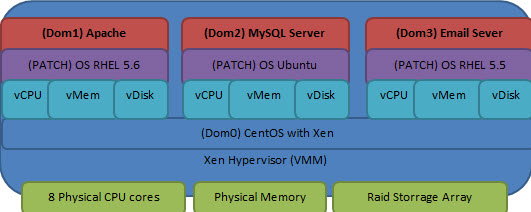
\includegraphics[width=3.5in]{images/VirtualizationExample.jpg}
  \end{center}

  \caption{\small In this example there are 3 paravirtualized guests (DomU) running on a Xen Server.  The Xen hypervisor and Dom0 divide, share, and overcommit the physical resources between the 3 guest domains.  Each guest has access to virtual resources and not physical hardware.}
  \label{fig-VirtualizationExample.pdf}
\end{figure}

\indent The problem this introduces is in performing profiling and analysis of this additional layer of abstraction for the guest systems.  The hypervisor, or Virtual Machine Manager, adds to the already complex existing layers (Application, OS, and Hardware) one must analyze when an application performs sub-optimally.  How can a system administrator determine if the problem is in the application, OS, hypervisor, hardware, or an unrelated guest virtual machine on the same physical host system?  In a traditional environment there can be 'interference' \cite{paul}or ‘system noise' caused by these layers, which attributes to poor application performance.  The hypervisor as well as multiple other guest virtual machines which compete for system resources add to this outside interference, which is undetectable from a guest VM, and therefore undetectable by the guest applications.

\indent This paper we show that using existing profiling tools and measuring changes in system runtime data in the guests and VMM we are now able to determine the layer of the complex software stack that attributes to a sub-optimal running application in a virtual environment.  Additionally, we can determine which system resource (memory, CPU, or IO) needs to be modified or is used inefficiently.

\indent This project will add the following contributions for virtualization:
\begin{enumerate}
\item Define the layers of abstraction in various virtual environments.
\item Define the system resources which attributes to application problem from I/O, memory, or CPU problems.
\item Framework to Identify the counters, metrics, and envirement at each layer which contributes to I/O contention.
\item Example tool which dynamically analyzes runtime interference and identifies the layer which experiences I/O contention.
\item Introduce \emph{disk pinning} for virtualization where separate physical disks are assigned to individual virtual servers.
\end{enumerate}


